\chapter{Umsetzung}
\label{chap:implementation}

Nachdem die Ziele der angestrebten TypeScript-Migration charakterisiert und die Anforderungen an den geplanten Transpiler ausgeführt wurden, soll im Folgenden der Entwurf und die Details der Implementierung umfassend betrachtet werden. In Abschnitt~\ref{subsec:js-transpilers} wurden bereits die verbreitetsten Werkzeuge zur Transformation von JavaScript-Quelltexten vorgestellt und verglichen. Auf Basis dieser Gegenüberstellung wurde schließlich Babel~\autocite{BABEL} als Grundlage der vorliegenden Umsetzung des Transpilers von Flow nach TypeScript gewählt.

\section{Software-Architektur}
\label{sec:software-architecture}

Mit der Entscheidung den Übersetzer als Babel-Plugin zu implementieren, ist dessen Grundarchitektur bereits in Teilen festgelegt, da alle Plugins die vorgegebenen Programmschnittstellen von Babel erfüllen müssen. Bevor auf Einzelheiten der Umsetzung näher eingegangen wird, soll zunächst der grundsätzliche Aufbau der Anwendung skizziert werden. Abbildung~\ref{fig:architecture-overview} verschafft einen Überblick über die verschiedenen Komponenten des Systems und deren Beziehung zueinander.

\begin{figure}[tbp]
  \centering
  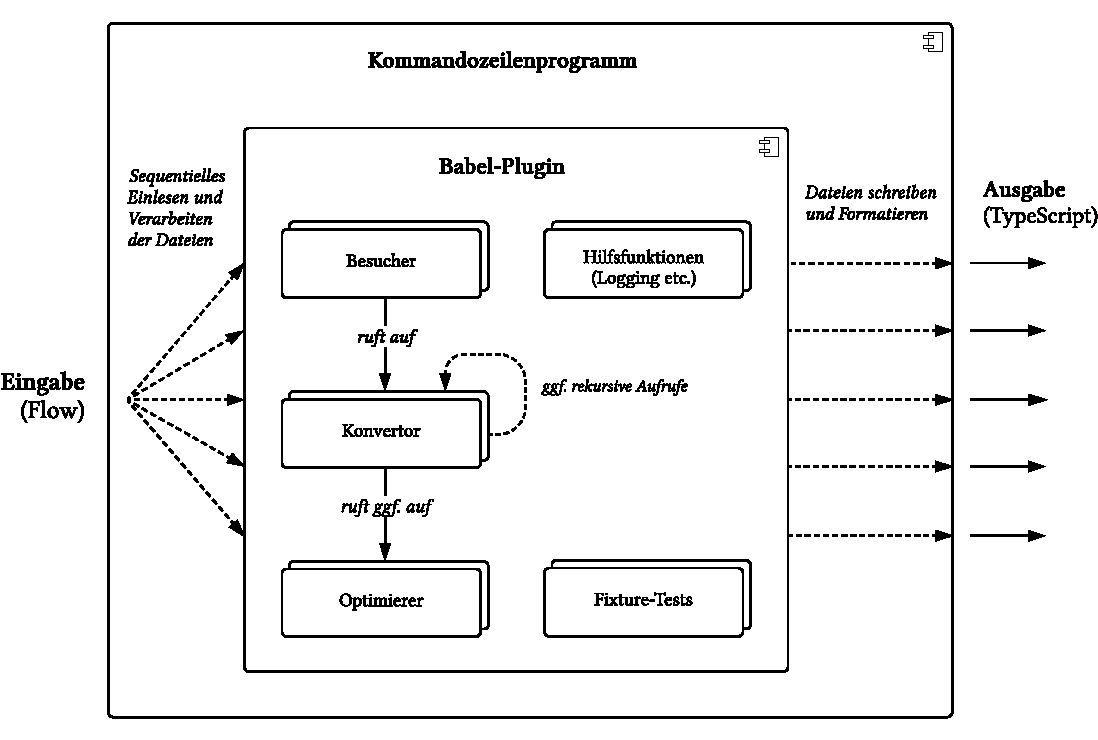
\includegraphics[width=0.92\textwidth]{src/4_Umsetzung/fig/architecture-overview.pdf}
	\caption{Überblick über die Komponenten des Transpilers.}
	\label{fig:architecture-overview}
\end{figure}

Die Architektur gliedert sich in zwei Teile: Ein Kommandozeilenprogramm stellt die Benutzerschnittstelle dar, welche die Eingabe-Verzeichnisse bzw. -Dateien als Argument entgegen nimmt und verschiedene Optionen bereit stellt, um das Verhalten der Übersetzung zu beeinflussen (siehe Tabelle~\ref{tab:cli-options}). Die zweite Komponente ist das Babel-Plugin, das die Transpilierung des Flow-Codes nach TypeScript realisiert. Das Kommandozeilenprogramm liest sukzessive alle Eingabeverzeichnisse bzw. -dateien ein und startet intern die Übersetzung des Quelltexts durch Babel. Hierfür wird das vorliegende Plugin geladen und dieses auf die Eingabe angewendet. Danach kann der generierte TypeScript-Code formatiert und in Dateien oder auf die Standardausgabe geschrieben werden.

Das Plugin setzt sich aus verschiedenen Unterkomponenten zusammen: Auf oberster Ebene befinden sich die Besucherfunktionen\footnote{Vgl. Abschnitt~\ref{subsection:babel-plugins}.}. Diese adressieren alle Pfade des abstrakten Syntaxbaums des Eingabeprogramms, die Flow-Syntax darstellen. Bei der Traversierung des Baums durch Babel werden alle zugehörigen Pfadknoten durch Ausführung verschiedener \emph{Konverter} in äquivalentes TypeScript übersetzt. Dabei kann es während der Verarbeitung zu rekursiven Aufrufen weiterer Besucher bzw. Konverter kommen. In einigen Fällen liegen weiterhin Methoden zur Optimierung des Transformationsresultats vor, die nach der Konvertierung gegebenenfalls angewandt werden. Darüber hinaus beinhaltet das Plugin Hilfsfunktionen, um verschiedene Aufgaben, wie beispielsweise die Ausgabe von Fehlern und Warnungen zu ermöglichen. Schließlich enthält das Plugin eine Vielzahl von Modultests (\textit{Unit tests}), welche die korrekte Funktionalität aller Komponenten überprüfen.

\section{Entwicklungsprozess}

% Bevor die konkrete Implementierung des Transpilers betrachtet wird, sollen zunächst zwei Aspekte des Entwicklungsprozesses, die diesen wesentlich unterstützt haben, näher betrachtet werden.

\subsection{Testgetriebene Entwicklung}

Die korrekte Übersetzung der Flow-Typen nach TypeScript ist die wichtigste Anforderung an den Transpiler\footnote{Vgl. Anforderung \ref{subsection:requirement:correct-translation}.}. Essentiell ist daher die Bereitstellung zuverlässiger Testmechanismen, um Software-Regressionen während der Entwicklungphase frühzeitig festzustellen. Unter Regressionen werden Bugs verstanden, die nach bestimmten Ereignissen wie der Implementierung weiterer Features oder Software-Upgrades unvorhergesehen in bereits getesteten Modulen auftreten~\autocite[218]{DOR:SOFTWARE_TEST}. Zur Erfüllung der Anforderung wurde der Ansatz der \emph{testgetriebenen Entwicklung}\footnote{engl. \textit{Test-driven development (TDD).}} gewählt, um die korrekte Funktionalität und Wechselwirkung aller Bestandteile des Transpilers kontinuierlich zu überprüfen. Die testgetriebene Entwicklung hat ihren Ursprung im Vorgehensmodell \enquote{\textit{Extreme Programming}}~\autocite{JEFFRIES:EXTREME_PROGRAMMING} aus der Software-Entwicklung und sieht im Gegensatz zu klassischen, seriellen Vorgehensweisen wie dem Wasserfall-Modell vor, dass sämtliche Testfälle eines Features bereits \emph{vor} dessen Umsetzung geschrieben werden müssen~\autocite{BECK:EXTREME_PROGRAMMING}. Die Vorteile dieser Methodik ist die Gewährleistung einer hohen Testabdeckung~\autocite[90]{BECK:TDD} und die Erzielung einer Implementierung, welche die Anforderungen \emph{vollständig} erfüllt, sofern die Testfälle sorgfältig konstruiert werden~\autocite[214]{BECK:TDD}. Wenn die Testfälle erst nach der Programmierung der Software angelegt werden, besteht die Gefahr, dass diese lediglich die tatsächlich umgesetzten Features betrachten, jedoch nicht den ursprünglichen, möglicherweise abweichenden Anforderungen gerecht werden.

Der Testaufbau wurde wie folgt konzipiert: Pro Modul wird ein Verzeichnis mit einer Ein\-gabe- und einer Ausgabe-Datei angelegt. Die Eingabe enthält dabei reguläres JavaScript, das mit Flow typisiert wurde, und die Ausgabe den äquivalenten, manuell übersetzten TypeScript-Code. In den Dateien können beliebig viele Testfälle einer Kategorie spezifiziert werden, um ein bestimmtes Feature des Transpilers zu erproben. Derartige Dateien oder Objekte, die der Initialisierung von Modultests dienen, werden oft als \enquote{Fixtures} bezeichnet~\autocite{OLAN:2003}. Durch die bewusste Aufteilung auf zwei unabhängige Dateien kann die inhärente Validität der jeweiligen Quelltexte besser gewährleistet werden, da diese jeweils mittels Flow bzw. TypeScript auf Typfehler überprüft werden können. Hierdurch wird vermieden, dass bereits die Testfälle fehlerhaft hinsichtlich der Syntax bzw. der Typisierung erstellt werden. Würden die Quelltexte als Zeichenketten innerhalb des Testprogramms angegeben werden, so wäre eine derartige Prüfung durch das statische Typsystem nicht möglich.

Die Testdurchführung kann nun wie folgt umgesetzt werden: Der Transpiler wird auf die Eingabedatei angewandt und der auf diese Weise generierte Code wird anschließend Zeile für Zeile mit der erwarteten Ausgabe exakt verglichen. Um dies zu erreichen wurde ein Skript geschrieben, welches das Verzeichnis mit den Modultests einliest, die Transpilierung anstößt und anschließend den zeilenweisen Vergleich durch das Test-Framework \textit{Jest}~\autocite{SOFTWARE:JEST} durchführt. Das angegebene Verzeichnis kann dabei wie in Quelltext~\ref{code:fixture-tests} veranschaulicht beliebig tief verschachtelte Unterverzeichnisse mit Fixture-Dateien enthalten.

\bigbreak
\begin{listing}[htb]
\begin{textcode}
tests/fixtures
└── types
    ├── any
    │     ├── input.js
    │     └── output.ts
    ├── …
    └── utility
        └── call
            ├── input.js
            └── output.ts
\end{textcode}
\listingvspace
\caption{Fixture-Dateien zum Test der korrekten Transpilierung der Flow-Typen.}
\label{code:fixture-tests}
\end{listing}

Während der Entwicklung des Transpilers wurden nach und nach Modultests für alle Funktionen des Programms angelegt. Überprüft wird dabei die Übersetzung aller Flow-Typen, die Korrektheit weiterer Optimierungen und die Formatierung der Ausgabe. Weiterhin wurden Tests zur Erprobung des Kommandozeilenprogramms und der allgemeinen Hilfsfunktionen geschrieben. Damit Regression während der fortlaufenden Entwicklung unmittelbar festgestellt werden, werden die Tests nach Einchecken von Änderungen in das Versionverwaltungssystem automatisch ausgeführt (\textit{kontinuierliche Integration}). Insgesamt sind 972 Testfälle\footnote{Anmerkung: Diese hohe Zahl ist darin begründet, dass größtenteils Fixture-Tests umgesetzt wurden und jeder Zeilenvergleich hierbei als ein Test betrachtet wird.} entstanden und es wurde eine Testabdeckung von 94,4\% erreicht.
% TODO: check those numbers at the end

\subsection{Statische Typisierung von Babel}

Der gesamte Transpiler, also sowohl das Babel-Plugin, als auch das zugehörige Kommandozeilenprogramm wurden in TypeScript implementiert. Neben den allgemeinen, bereits ausgeführten Vorteilen statischer Typsysteme, ist der primäre Grund hierfür, dass so die durch Babel bereitgestellten Typdeklarationen benutzt werden können. Diese unterstützen die Entwicklungsprozess enorm, weil die Attribute aller Knoten des abstrakten Syntaxbaums von Babel und die Signatur sämtlicher Methoden durch die Typisierung genau spezifiziert sind. Somit kann während der Entwicklung durch den TypeScript-Compiler unmittelbar festgestellt werden, ob fehlerhafte Aufrufe von Bibliotheksfunktionen oder anderweitige Typverletzungen bestehen. Quelltext~\ref{code:babel:static-types} zeigt den Aufbau dieser Typdeklarationen von Babel am Beispiel des Knotens eines Typalias.

\bigbreak
\begin{listing}[htb]
\begin{textcode}
interface TypeAlias extends BaseNode {
  type: "TypeAlias";
  id: Identifier;
  typeParameters: TypeParameterDeclaration | null;
  right: FlowType;
}
\end{textcode}
\listingvspace
\caption{Externe Definition des Typen des AST-Knotens \textit{TypeAlias} in Babel.}
\label{code:babel:static-types}
\end{listing}

Da bekannt ist welcher TypeScript-Knoten zu konstruieren ist, um einen Flow-Ausdruck zu übersetzen, ist durch die Typisierung der Methoden zur Erstellung dieses AST-Knotens auch bekannt, welche Typen die Funktionsargumente erwarten. Die Implementierung von Transformationen wird hierdurch erheblich vereinfacht, da so lediglich die Attribute des Ursprungsknoten korrekt auf den Typ des jeweiligen Funktionsparameters abgebildet werden müssen. Es hat sich während der Entwicklung gezeigt, dass eine derartige Einschränkung durch die Typisierung sehr hilfreich ist: Wenn keine Typfehler mehr vorliegen, ist die Transformation erfahrungsgemäß mit hoher Wahrscheinlichkeit korrekt.

\section{Implementierung als Babel-Plugin}

\subsection{Ablauf der Transpilierung}

Abbildung~\ref{fig:activity-diagram-plugin} auf Seite~\pageref{fig:activity-diagram-plugin} veranschaulicht den konzeptionellen Aufbau der Transpilierung innerhalb des Babel-Plugins anhand eines Aktivitätsdiagramms. Aktivitätsdiagramme entstammen der Modellierungssprache \textit{Unified Modeling Language} (UML)~\autocite{OMG:UML} und veranschaulichen die Arbeitsweise von Prozessen innerhalb eines Software-Systems. Zu Beginn wird das Plugin wie im Grundlagenteil in Quelltext~\ref{code:babel-plugin-definition} bereits exemplarisch gezeigt initialisiert, das heißt es wird eine Abbildung der Flow-Knotentypen des abstrakten Syntaxbaums auf Besucher"=Funktionen definiert. Diese realisieren die Transformation aller Flow-Typannotationen in entsprechende TypeScript-Syntax.
Weiterhin werden die Abhängigkeiten des Plugins spezifiziert. Dabei handelt es sich um weitere vorgegebene Babel-Plugins, die benötigt werden, um die Syntax von Flow, JSX und vorläufiger ECMAScript-Erweiterungen einlesen zu können. Auf Grundlage der konkreten Anforderungen bei TeamShirts wurden externe Plugins für folgende Erweiterungen aktiviert:

\begin{itemize}
  \item \textit{Class field declarations for JavaScript}~\autocite{ES_PROPOSAL:CLASS_FIELDS}
  \item \textit{JavaScript decorators}~\autocite{ES_PROPOSAL:DECORATORS}
  \item \textit{Dynamic imports}~\autocite{ES_PROPOSAL:DYNAMIC_IMPORTS}
\end{itemize}

\begin{figure}[p]
  \centering
  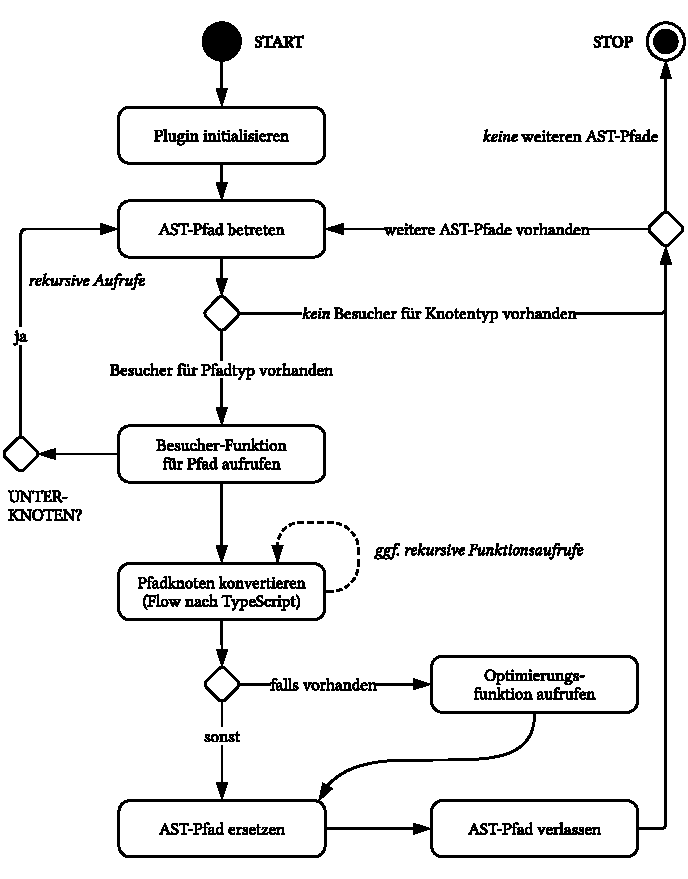
\includegraphics[width=0.85\textwidth]{src/4_Umsetzung/fig/activity-diagram-plugin.pdf}
  \caption{Aktivitätsdiagramm des Transpilers (Babel-Plugin).}
  \label{fig:activity-diagram-plugin}
\end{figure}

Nach der Initialisierung beginnt die rekursive Traversierung des abstrakten Syntaxbaums der Eingabe, um diese umzuformen. Die Datenstruktur des Syntaxbaums wird von Babel durch Parsen des Flow-Programms aufgebaut. Jeder Knoten des Baums wird dabei zunächst \enquote{betreten} und daraufhin wieder \enquote{verlassen}~\autocite{BABEL:HANDBOOK}. Knoten werden verlassen, wenn bei der Beschreitung eines Pfads ein Blatt des Baums erreicht wird und die Traversierung daraufhin auf der höherliegenden Ebene fortgesetzt wird.

Sofern eine Besucherfunktion für den aktuellen Knotentyp existiert, wird diese mit dem zugehörigen Pfad als Argument aufgerufen. Ansonsten wird das nächste Element des Syntaxbaums betreten bzw. die Transpilierung beendet, falls keine weiteren Knoten bestehen. Wenn innerhalb der Besucherfunktion festgestellt wird, dass Kindknoten vorliegen, so wird deren Pfad rekursiv beschritten. Andernfalls wird der Konverter für diesen speziellen Knotentyp ausgeführt, sodass der momentane Pfad anschließend mit dem auf diese Weise berechneten TypeScript-Gegenstück ersetzt werden kann. Gleichzeitig werden für einige Knotenarten Optimierungsfunktionen aufgerufen. Diese korrigieren beispielsweise fehlerhaft verwendete Typen und sind auf die konkreten JavaScript-Projekte abgestimmt. Da viele der Typannotationen von Flow zusammengesetzt sind (z.~B. \textit{Union}, \textit{Intersection}, usw.), werden diese Ausdrücke durch mehrere, rekursive Aufrufe von Konvertern umgeformt. Zuletzt wird der momentane Pfad verlassen und die Prozedur beginnt von neuem, sofern weitere Elemente im abstrakten Syntaxbaum vorliegen. Sobald das gesamte Programm und damit sämtliche Flow-Typen übersetzt wurden, kann die TypeScript-Ausgabe mittels des Babel Codegenerators~\autocite{BABEL:GENERATOR} erzeugt werden.

\subsection{Transpilierung der Flow-Typen}

Im Folgenden soll nun genauer auf den Kern des Transpilers, die Konverterfunktionen, eingegangen werden. Aufgrund der großen Zahl von Flow-Typen kann nicht die vollständige Umsetzung aller Transformationen und sämtlicher Grenzfälle ausführlich behandelt werden, da dies den Umfang der Arbeit überschreiten würde. Deshalb wird nachfolgend lediglich ein Überblick über alle Übersetzungen gegeben. Zur Verbesserung der Anschaulichkeit wurden darüber hinaus einige repräsentative Beispiele ausgewählt, anhand derer das Prinzip der Transpilierung detaillierter erläutert wird, indem die zugrunde liegende Implementierung betrachtet wird. Die genaue Implementierung aller Transformationen und die Behandlung der Spezialfälle kann mittels des veröffentlichten Quelltexts des Transpilers~\autocite{REFLOW_GITHUB} nachvollzogen werden.

\subsubsection{Transpilierung der Basistypen}

Die Mehrheit der in Tabelle~\ref{tab:flow-base-types} vorgestellten Basistypen von Flow kann innerhalb des Plugins simpel übersetzt werden, da der entsprechende Typ in TypeScript die gleiche Syntax besitzt oder sich lediglich das Schlüsselwort unterscheidet. Von den 30 Basistypen gehören 18 zu dieser einfachen Kategorie. Die verbleibenden zwölf Typen erfordern komplexere Knotentransformationen, um die Annotationen in entsprechende TypeScript-Konstrukte umzuwandeln.

\paragraph{Simple Übersetzungen}

Tabelle~\ref{tab:transformation-base-types-simple} auf Seite~\pageref{tab:transformation-base-types-simple} listet die 18 Flow-Typen auf, die simpel übersetzt werden können und zeigt beispielhaft deren Entsprechung in TypeScript. Abgesehen von den zwei kursiv hervorgehobenen Zeilen ist die Syntax in TypeScript identisch mit der ursprünglichen Notation der Typen in Flow. Dennoch müssen auch diese Elemente des abstrakten Syntaxbaums während der Transpilierung in ihr korrektes Gegenstück umgewandelt werden, da eine Kombination von Flow- und TypeScript-Knoten gemäß der Spezifikation~\autocite{BABEL:PARSER_SPEC} von Babel unmöglich ist. Diese Einschränkung wird zur Laufzeit durch die im Plugin eingesetzte Bibliothek \code{@babel/types}\,\autocite{BABEL:TYPES} sicher gestellt. Durch die Verwendung von TypeScript und der gegebenen Typisierung von Babel, werden Typfehler dieser Art wie erwähnt ohnehin bereits vor Ausführung des Transpilers statisch erkannt.

\bigbreak
\begin{table}[tbh]
  \footnotesize
  \begin{tabu} to \textwidth {@{}lCCX@{}}
    \midrule
    \libertineSB{Basistyp}  & \libertineSB{Flow}            & \libertineSB{TypeScript}         & {} \\
    \midrule
    Any type                & any                           & any                              & {} \\
    Array type              & Array<number>                 & Array<number>                    & {} \\
    Array type (shorthand)  & number[]                      & number[]                         & {} \\
    Boolean literal type    & true                          & true                             & {} \\
    Boolean type            & boolean                       & boolean                          & {} \\
    \textit{Empty type}     & empty                         & never                            & {} \\
    Intersection type       & type Intersection = T1 \& T2  & type Intersection = T1 \& T2     & {} \\
    \textit{Mixed type}     & mixed                         & unknown                          & {} \\
    Null literal type       & null                          & null                             & {} \\
    Number literal type     & 42                            & 42                               & {} \\
    Number type             & number                        & number                           & {} \\
    String literal type     & \str{literal}                 & \str{literal}                    &  {} \\
    String type             & string                        & string                           & {} \\
    This type               & this                          & this                             & {} \\
    Tuple type              & {[}Date, number{]}            & {[}Date, number{]}               & {} \\
    Type alias              & type Type = <FlowType>        & type Type = <TypeScriptType>     & {} \\
    Union type              & number | null                 & number | null                    & {} \\
    Void type               & void                          & void                             & {} \\
    \midrule
  \end{tabu}
  \caption{Übersicht über simple Transformationen der Basistypen von Flow.}
  \label{tab:transformation-base-types-simple}
\end{table}



\bigbreak
\begin{listing}[htb]
\begin{textcode}
// @flow                              // TypeScript
type Alias = mixed;                  type Alias = unknown;
\end{textcode}
\listingvspace
\caption{Beispiel für die Übersetzung simpler Flow-Typen.}
\label{code:example-simple}
\end{listing}

Anhand eines Beispiels wird nachfolgend der Ablauf einer einfachen Übersetzungen und das grundsätzliche Vorgehen bei der Implementierung erläutert. Quelltext~\ref{code:example-simple} zeigt links das mit Flow typisierte Ursprungsprogramm und rechts den äquivalenten TypeScript-Code. In der zweiten Zeile wird ein Typalias definiert, welcher auf den Typ
\code{mixed}\footnote{Siehe~\autocite[Mixed Types]{FLOW:TYPE_ANNOTATIONS}.} verweist. Gemäß Tabelle~\ref{tab:transformation-base-types-simple} ist der korrespondierende TypeScript-Typ \code{unknown}. Um die notwendigen Schritte der Transformation zu erkennen, ist es hilfreich die abstrakten Syntaxbäume des ursprünglichen und angestrebten Quelltexts zu vergleichen. Abbildung~\ref{ast:example-simple} zeigt den Syntaxbaum des Beispiels für Flow (links) und TypeScript (rechts)\footnote{Anmerkung: Zur Vereinfachung der Nachvollziehbarkeit werden nur wesentliche Teile des Syntaxbaums gezeigt. Tatsächlich besitzen alle Knoten weitere Attribute, die hier jedoch irrelevant sind.}. Die Typen der verschiedenen Knoten werden dabei in \texttt{Festbreitenschrift} abgedruckt, konkrete Werte wie beispielsweise der Name von Bezeichnern dagegen in Serifenschrift. Die Kantenbeschriftungen stehen für Attribute der Knoten.

\bigbreak
\begin{figure}[htb]
  \centering
  \small
  \ttfamily
  \begin{subfigure}{.5\textwidth}
    \centering
    \begin{forest}
      for tree = {l=1.6cm, s sep=0.5cm}
      [Program
        [TypeAlias, edge label={node[midway,fill=white,font=\scriptsize\ttfamily]{body}}
          [Identifier, edge label={node[midway,fill=white,font=\scriptsize\ttfamily]{id}}
            [\textrm{Alias}, edge label={node[midway,fill=white,font=\scriptsize\ttfamily]{name}}]
          ]
          [MixedTypeAnnotation, edge label={node[midway,fill=white,font=\scriptsize\ttfamily]{right}}]
        ]
      ]
    \end{forest}
  \end{subfigure}%
  \begin{subfigure}{0.5\textwidth}
      \centering
      \begin{forest}
        for tree = {l=1.6cm, s sep=1cm}
        [Program
          [TSTypeAliasDeclaration, edge label={node[midway,fill=white,font=\scriptsize\ttfamily]{body}}
            [Identifier, edge label={node[midway,fill=white,font=\scriptsize\ttfamily]{id}}
              [\textrm{Alias}, edge label={node[midway,fill=white,font=\scriptsize\ttfamily]{name}}]
            ]
            [TSUnknownKeyword, edge label={node[midway,fill=white,font=\scriptsize\ttfamily]{typeAnnotation}}]
          ]
        ]
      \end{forest}
  \end{subfigure}
  \vspace{0.25cm}
  \caption{Abstrakter Syntaxbaum für die Deklaration eines Typalias in Flow und TypeScript.}
  \label{ast:example-simple}
\end{figure}

Die zwei Bäume sind sich sehr ähnlich: In der Wurzel der Datenstruktur befindet sich bei allen durch Babel eingelesenen Quelltexten der \code{Program}-Knoten. Dessen Kindknoten repräsentiert die Deklaration des Typalias aus der zweiten Zeile. Der Typ dieses Knotens ist \code{TypeAlias} in Flow und \code{TSTypeAliasDeclaration} in TypeScript. Auf der linken Seite der Anweisung steht dabei der Bezeichner des Alias und auf der rechten Seite der zugewiesene Datentyp. Da im ursprünglichen Code eine \code{MixedTypeAnnotation} vorliegt, muss dieser Knoten in TypeScript zu \code{unknown} (\code{TSUnknownKeyword}) übersetzt werden, um einen bedeutungsgleichen Ausdruck zu erzeugen. In diesem konkreten Fall sind die zwei notwendigen Transformationschritte damit folgende:

\begin{itemize}
  \item Übersetzung aller \code{TypeAlias}-Knoten nach \code{TSTypeAliasDeclaration}
  \item Übersetzung aller \code{MixedTypeAnnotation}-Knoten nach \code{TSUnknownKeyword}
\end{itemize}

Da ein \emph{beliebiger} Flow-Typ auf der rechten Seite des Typalias stehen kann, muss bei dessen Transpilierung auch der zugewiesene Typ allgemeingültig umgewandelt werden können. Es wurde deshalb eine Funktion implementiert, die alle Flow-Typen universell auf ihr TypeScript-Gegenstück abbildet. Deren vereinfachter Aufbau ist wie folgt:

\bigbreak
\begin{listing}[htb]
\begin{textcode}
function convertFlowType(node: FlowType): TSType {
  switch (node.type) {
    case 'ArrayTypeAnnotation':
      return tsArrayType(convertFlowType(node.elementType));
    // …
    case 'InterfaceTypeAnnotation':
      return convertInterfaceTypeAnnotation(node);
    // …
    case 'MixedTypeAnnotation':
      return tsUnknownKeyword();
  }
}
\end{textcode}
\listingvspace
\caption{Universelle Transpilierung aller Flow-Typen nach TypeScript durch zentrale Umwandlungsfunktion.}
\label{code:convert-flow-type}
\end{listing}

Der zweite Schritt der AST-Transformation für das Beispiel, also die Übersetzung des \code{mixed}-Schlüsselworts nach \code{unknown}, wird in Zeile 10 umgesetzt. Durch Aufruf der durch Babel gegebenen Bibliotheksfunktion \code{tsUnknownKeyword()} kann ein neuer AST-Knoten erzeugt werden, der das entsprechende Schlüsselwort in TypeScript darstellt. Babel stellt für sämtliche Knotentypen Methoden mit diversen Parametern bereit, mittels derer alle Elemente des Syntaxbaums erstellt werden können\footnote{Siehe~\autocite{BABEL:TYPES}.}.

In Zeile 4 wird ein weiteres, wichtiges Konzept innerhalb des Transpilers exemplarisch aufgezeigt: Für Knoten des Typs \code{ArrayTypeAnnotation} wird die Umwandlungsfunktion \emph{rekursiv} aufgerufen, da auch hier beliebige Flow-Typen Argument des Feldtyps sind. Wie die weiteren Ausführungen zeigen werden, spielt die obige Umwandlungsmethode eine zentrale Rolle innerhalb des Transpilers, da sie in nahezu allen Konvertern aufgerufen wird. Zeile sieben verdeutlicht schließlich, dass nicht alle Knoten so einfach wie das Typalias aus dem Beispiel umgewandelt werden können, da der Aufbau vieler Typen komplexer ist. Die Transformation dieser Knoten wird durch jeweilige Konverterfunktionen separat durchgeführt.

\paragraph{Komplexere Übersetzungen}

Die Übersetzung der zwölf komplexen Flow"=Datentypen ist in Tabelle~\ref{tab:transformation-base-types-complex} exemplarisch dargestellt. Im Gegensatz zu den simplen Transformationen unterscheidet sich die Syntax des Ausgabequelltexts hier zum Teil deutlich und es müssen bei der Transpilierung Spezial- und Grenzfälle beachtet werden, um korrekten TypeScript-Code zu erzeugen. Zum Beispiel erlaubt Flow den Typ einer Funktion, die eine Zeichenkette und eine Zahl als Parameter entgegen nimmt, wie folgt anzugeben:
\\[.5\baselineskip]
{\small\texttt{type FunctionType = (string, argName: number) => void;}}
\\[.5\baselineskip]
Während die Benennung der Funktionsargumente in Flow optional ist, ist diese in TypeScript verbindlich. Infolgedessen müssen Parameter während der Übersetzung von Funktionstypen nach TypeScript gegebenenfalls automatisch benannt werden, da andernfalls fehlerhafte Syntax entstünde (vgl. Zeile 2 in Tabelle~\ref{tab:transformation-base-types-complex}).

\bigbreak
% TODO sync with chapter 2, maybe line breaks
\begin{longtabuenv}
\begin{longtabu} to \textwidth {@{}lCCX@{}}
  \captionlistentry{Übersicht über komplexe Transformationen der Basistypen von Flow.} \\
  \midrule
  \libertineSB{Basistyp} & \libertineSB{Flow} & \libertineSB{TypeScript} & {} \\
  \midrule
\endfirsthead
  \midrule
  \libertineSB{Basistyp} & \libertineSB{Flow} & \libertineSB{TypeScript} & {} \\
  \midrule
\endhead
  \midrule
  \caption[]{Übersicht über komplexe Transformationen der Basistypen von Flow.}
\endfoot
  Exact object type          & \{| prop: any |\}                &   \{ prop: any \}                      & {} \\
  Function type              & (string, \{\}) => number         &   (p1: string, p2: \{\}) => number     & {} \\
  Generic type annotation    & let v: <{}FlowType>{}            &   let v: <{}TSType>{}                  & {} \\
  Generics                   & type Generic<{}T: Super> = T     &   type Generic<{}T extends Super> = T  & {} \\
  Interface type             & interface I \{ +prop: number \}  &   interface I \{ readonly: number \}   & {} \\
  Nullable type (Maybe type) & ?number                          &   number | null | undefined            & {} \\
  Object type                & \{ {[}string{]}: number \}       &   \{ {[}key: string{]}: number \}      & {} \\
  \textit{Opaque type}       & opaque type Opaque = number      &   type Opaque = number                 & {} \\
  Type cast expresssion      & (variable: string)               &   (variable as string)                 & {} \\
  Type export                & export type T = number | null    &   export T = number | null             & {} \\
  Type import                & import type T from \str{./types} &   import T from \str{./types}          & {} \\
  Typeof type                & typeof undefined                 &   undefined                            & {}
  \label{tab:transformation-base-types-complex}
\end{longtabu}
\end{longtabuenv}


Anhand des Typs \enquote{Nullable} soll das Vorgehen bei der Transformation eines komplizierteren Knoten erläutert werden\footnote{Anmerkung: Es wurde ein verhältnismäßig unkompliziertes Beispiel ausgewählt, weil die Ausführung anderer deutlich komplexerer Fälle nicht in prägnanter Form dargelegt werden könnte.}. Dieser Typ wird in der Flow-Dokumentation auch als \enquote{\textit{Maybe type}} bezeichnet und wird für die Typisierung optionaler, möglicherweise undefinierter Werte verwendet\footnote{Siehe~\autocite[Maybe Types]{FLOW:TYPE_ANNOTATIONS}.}. Konkret stellt der Typ die Vereinigung aus dem angegebenen Datentyp, \code{null} und \code{undef\/ined} dar. In TypeScript existiert keine direkte Entsprechung, aber es kann trivial ein äquivalenter Vereinigungstyps angegeben werden. Quelltext~\ref{code:example-complex} zeigt analog zum vorherigen Beispiel die jeweilige Deklaration eines Typalias in Flow (links) und TypeScript (rechts), das auf diesen Datentyp verweist.

\bigbreak
\begin{listing}[htb]
\begin{textcode}
// @flow                               // TypeScript
type MaybeNumber = ?number;           type MaybeNumber = number | null | undefined;
\end{textcode}
\listingvspace
\caption{Beispiel für die Übersetzung komplexer Flow-Typen.}
\label{code:example-complex}
\end{listing}

Wie zuvor sollen zunächst die abstrakten Syntaxbäume der Ein- und Ausgabe verglichen werden, um die Einzelschritte der Transpilierung aufzuzeigen. Das Typalias ist analog zum vorherigen Beispiel und dient lediglich der Herstellung korrekter Syntax. Entscheidend ist der zugewiesene Typ des Alias im rechten Teilbaum: Bei Flow liegt hier eine \code{NullableTypeAnnotation} vor, der den Datentyp für Zahlen als Argument erhält. Auf Seite von TypeScript steht dagegen der Knoten des Vereinigungstyps (\code{TSUnionType}). Diesem ist eine Menge von Typen zugeordnet, die den äquivalenten Ausdruck bilden, indem der Zahlentyp mit den Typen für \code{null} und \code{undefined} vereint wird.

\bigbreak
\begin{figure}[htb]
  \footnotesize
  \ttfamily
  \begin{minipage}{.47\textwidth}
    \centering
    \vspace{-0.87cm}
    \begin{forest}
      for tree = {l=1.6cm, s sep=0.5cm}
      [Program
        [TypeAlias, edge label={node[midway,fill=white,font=\scriptsize\ttfamily]{body}}
          [Identifier, edge label={node[midway,fill=white,font=\scriptsize\ttfamily]{id}}
            [\textrm{MaybeNumber}, edge label={node[midway,fill=white,font=\scriptsize\ttfamily]{name}}]
          ]
          [NullableTypeAnnotation, edge label={node[midway,fill=white,font=\scriptsize\ttfamily]{right}}
            [NumberTypeAnnotation, edge label={node[midway,fill=white,font=\scriptsize\ttfamily]{typeAnnotation}}]
          ]
        ]
      ]
    \end{forest}
  \end{minipage}%
  \begin{minipage}{.53\textwidth}
    \centering
    \begin{forest}
      for tree = {l=1.6cm, s sep=1.25cm, align=center}
      [Program
        [TSTypeAliasDeclaration, edge label={node[midway,fill=white,font=\scriptsize\ttfamily]{body}}
          [Identifier, edge label={node[midway,fill=white,font=\scriptsize\ttfamily]{id}}
            [\textrm{MaybeNumber}, edge label={node[midway,fill=white,font=\scriptsize\ttfamily]{name}}]
          ]
          [TSUnionType, edge label={node[midway,fill=white,font=\scriptsize\ttfamily]{typeAnnotation}}
            [{TSNumberKeyword,\\ TSNullKeyword,\\ TSUndefinedKeyword}, align=left, s sep=0.5cm, edge label={node[midway,fill=white,font=\scriptsize\ttfamily]{types}}]
          ]
        ]
      ]
    \end{forest}
  \end{minipage}
  \vspace{0.25cm}
  \caption{Abstrakter Syntaxbaum für die Deklaration eines \enquote{Maybe type} in Flow (links) und TypeScript (rechts).}
  \label{ast:example-complex}
\end{figure}

Quelltext~\ref{code:convert-nullable-type} zeigt die entsprechende Implementierung. Zuerst wird in Zeile zwei das Argument des Typs \code{NullableTypeAnnotation} durch Aufruf der bereits gezeigten, zentralen Umwandlungsfunktion von Flow in den korrekten TypeScript-Typ übersetzt. Im vorliegenden Fall wird Flows \code{NumberTypeAnnotation} in das Gegenstück \code{TSNumberKeyword} überführt. Anschließend wird eine Liste aufgebaut, die aus diesem Datentyp und der Typen für \code{null} und \code{undefined} besteht. Zu Beachten sind hierbei zwei Spezialfälle: Einerseits darf der Nullwert nicht doppelt in die Liste aufgenommen werden, andererseits muss der Funktionstypen in dieser Situationen geklammert werden, um korrekte Syntax herzustellen. Eine Doppelung träte dann auf, wenn in Flow der wenig sinnvolle Typ \code{?null} verwendet wird. Zuletzt kann der Vereinigungstyp in TypeScript durch Aufruf der entsprechenden Hilfsfunktion, welche die Typliste als Argument erhält, erstellt und zurück geliefert werden.

\bigbreak
\begin{listing}[htb]
\begin{textcode}
function convertNullableTypeAnnotation(node: NullableTypeAnnotation): TSUnionType {
  const tsType = convertFlowType(node.typeAnnotation);
  const types = [
    ...(isTSNullKeyword(tsType)
      ? []
      : [isTSFunctionType(tsType) ? tsParenthesizedType(tsType) : tsType]),
    tsNullKeyword(),
    tsUndefinedKeyword(),
  ];

  return tsUnionType(types);
}
\end{textcode}
\listingvspace
\caption{Transpilierung eines \textit{Maybe types} in äquivalenten Vereinigungstyp in TypeScript.}
\label{code:convert-nullable-type}
\end{listing}

\subsubsection{Transpilierung der Hilfstypen}

Auch die in Abschnitt~\ref{subsection:flow:utility-types} eingeführten Hilfstypen von Flow können größtenteils äquivalent nach TypeScript überführt werden. Tabelle~\ref{tab:transformation-utility-types} auf Seite~\pageref{tab:transformation-utility-types} gibt einen Überblick über alle Übersetzungen. Für einige der Einträge gibt es in TypeScript bedeutungsgleiche Hilfstypen, andere können leicht durch Verwendung von Typoperatoren abgebildet werden.

Die Transformation der drei Abbildungstypen \textit{Object map}, \textit{Object map with key}, \textit{Tuple map} sowie \textit{Rest} wurde nicht umgesetzt, da kein TypeScript-Ausdruck gefunden werden konnte, der diesen exakt entspricht. Da die vorliegenden JavaScript-Projekte bei TeamShirts diese Hilfstypen jedoch ohnehin nicht verwenden, stellt dies kein Hindernis für die Migration dar. Die zwei Typen \textit{Subtype} und \textit{Supertype} sind in der Dokumentation von Flow als veraltet (\textit{deprecated}) markiert worden~\autocite{FLOW:UTILITY_TYPES}. Deshalb werden auch diese nicht transpiliert, sondern unverändert in die Ausgabe übernommen. Sollten in der Eingabe einer dieser fünf nicht unterstützen Hilfstypen auftreten, so wird während der Verarbeitung durch das Babel-Plugin eine detaillierte Warnung ausgegeben mit der Aufforderung den Ausgabequelltext an dieser Stelle manuell zu korrigieren. Auch der kursiv hervorgehobene Typ \textit{Existential type} wurde von Flow als obsolet gekennzeichnet, da er unsicher ist~\autocite{FLOW:LINT_RULE_REFERENCE}. Der Sinn dieses Typs ist die Angabe eines Platzhalters für Typen, die durch das statische Typsystem selbstständig inferiert werden sollen\footnote{Dies ist vergleichbar zum Schlüsselwort \code{auto} in C++~\autocite[151]{CPP11_SPEC}.}. Weil TypeScript einen derartigen Typ nicht unterstützt, wird dieser durch \code{any} ersetzt.

\bigbreak
\begin{table}[tbh]
  \footnotesize
  \begin{tabu} to \textwidth {@{}lCCX[l]@{}}
    \midrule
    \libertineSB{Hilfstyp}    & \libertineSB{Flow}     & \libertineSB{TypeScript} & \libertineSB{Anmerkung} \\
    \midrule
    Call                         &  \$Call<F, T...>        & ReturnType<F>              & {} \\
    Class                        &  Class<C>               & typeof T                   & {} \\
    Difference                   &  \$Diff<A, B>           & Omit<A, keyof B>           & {} \\
    Element type                 &  \$ElementType<T, K>    & T[k]                       & {} \\
    Exact                        &  \$Exact<O>             & O                          & {} \\
    Existential type             &  *                      & any                        & Verlust von Typinformation! \\
    Keys                         &  \$Keys<O>              & keyof O                    & {} \\
    None maybe type              &  \$NonMaybeType<T>      & NonNullable<T>             & {} \\
    \textit{Object map}          &  \$ObjMap<O, F>         & any                        & nicht implementiert \\
    \textit{Object map with key} &  \$ObjMapi<O, F>        & any                        & nicht implementiert  \\
    Property type                &  \$PropertyType<O, k>   & O[k]                       & {} \\
    Read only                    &  \$ReadOnly<O>          & ReadOnly<O>                & {} \\
    Read only array              &  \$ReadOnlyArray<A>     & ReadonlyArray<A>           & {} \\
    Rest                         &  \$Rest<A, B>           & Omit<A, Union<keyof B>{>}  & {} \\
    Shape                        &  \$Shape<O>             & Partial<O>                 & {} \\
    \textit{Tuple map}           &  \$TupleMap<T, F>       & any                        & nicht implementiert \\
    Values                       &  \$Values<O>            & O[keyof O]                 & {} \\
    \textit{Subtype}             &  \$Subtype<T>           & any                        & obsolet \\
    \textit{Supertype}           &  \$Supertype<T>         & any                        & obsolet \\
    \midrule
  \end{tabu}
  \caption{Übersicht über Transformationen der Hilfstypen von Flow.}
  \label{tab:transformation-utility-types}
\end{table}


Zu beachten gilt darüber hinaus, dass die Typparameter der Hilfstypen (\code{T}, \code{A}, \code{B} usw.) für beliebige, kompatible Flow-Typen stehen. Auch hier ruft die Implementierung intern die universelle Konvertierungsfunktion \code{convertFlowType()} auf, um alle Eingaben korrekt zu übersetzen.

\subsubsection{Transpilierung der Typdeklarationen}

Da der Transpiler Anspruch auf Vollständigkeit erhebt, müssen auch Typdeklarationen transformiert werden. Tabelle~\ref{tab:transformation-declarations} zeigt exemplarisch die verschiedenen Deklarationen und deren Gegenstück in TypeScript. Die Syntax ist hierbei ähnlich zu den simplen Basistypen oftmals identisch in Flow und TypeScript. Dennoch müssen die zugrunde liegenden Knoten des abstrakten Syntaxbaums übersetzt werden, da deren Repräsentation in TypeScript eigene Knotentypen besitzen. Interessant ist die Deklaration des Standard-Exports\footnote{Siehe~\autocite[377]{ECMASCRIPT:2019}.} eines Moduls in der zweiten Zeile. Während Flow hier den Export von Funktionen unterstützt, kann dies nicht unmittelbar in TypeScript abgebildet werden. Deshalb muss die Deklaration umgeformt werden. Der Wert der ursprünglichen Deklaration wird dabei einer neu erstellten Variablen (\code{\_default}) zugewiesen und kann anschließend als Argument des Exports verwendet werden. Somit entsteht ein äquivalenter Ausdruck.

\bigbreak
% TODO: Sync with chapter 2
\begin{longtabuenv}
\begin{longtabu} to \textwidth {@{}lCK@{}}
  \midrule
  \libertineSB{Deklaration} & \libertineSB{Flow} & \libertineSB{TypeScript} \\
  \midrule
\endhead
  \midrule
  \caption[]{Übersicht über Transformationen der Typdeklarationen von Flow.}
\endfoot
  \captionlistentry{Übersicht über Transformationen der Typdeklarationen von Flow.}
  Class       & declare class C \{\}                 & declare class C \{\}                     \\
  Export      & declare export default () => string  & const \_default: () => string;\newline export default \_default; \\
  Function    & declare function f(number): any      & declare function f(p: number): any       \\
  Interface   & declare interface I \{\}             & declare interface I \{\}                 \\
  Module      & declare module \str{esmodule} \{\}   & declare module \str{esmodule} \{\}       \\
  Type alias  & declare type T = number              & declare type T = number                  \\
  Variable    & declare var v: ?string               & declare var v: string | null | undefined
  \label{tab:transformation-declarations}
\end{longtabu}
\end{longtabuenv}


\subsection{Weitere Optimierungen}
\label{subsec:optimizations}

Bei der Erprobung des Transpilers mit den realen JavaScript-Projekten von TeamShirts wurde die Erfahrung gewonnen, dass neben der Transformation der Flow-Typen auch andere Änderungen des Quelltexts nötig sind, um eine Migration zu TypeScript erfolgreich durchzuführen. Zur Reduzierung händischer Nacharbeit, wurden das Plugin um Funktionen erweitert, die diese zusätzlichen Schritte automatisieren.

\subsubsection{Übersetzung von React Typimporten}
\label{subsec:react-type-import-mapping}

Die von TeamShirts eingesetzte Bibliothek \textit{React} stellt ähnlich wie Babel Typdeklarationen sowohl für Flow, als auch für TypeScript bereit. Diese Typen können importiert und anschließend in den eigenen Typannotation verwendet werden. Leider wurden die korrespondierenden React-Typen in den Definitionen für Flow und TypeScript unterschiedlich benannt. Während einer der Typen in Flow beispielsweise \code{Node} heißt, ist dessen Bezeichnung in TypeScript \code{ReactNode}. Würden die Typimporte unverändert übernommen werden, so entstünden in der Ausgabe Typfehler, da der importierte Typ unter TypeScript nicht existiert.

\bigbreak
\begin{listing}[htb]
\begin{textcode}
// @flow                                        // TypeScript
import React, { type Node } from 'react';       import React, { ReactNode } from 'react';
type FunctionType = () => Node;                 type FunctionType = () => ReactNode;
\end{textcode}
\listingvspace
\caption{Import und Benutzung des durch die Bibliothek \textit{React} extern definierten Typs \enquote{Node}.}
\label{code:react-imports}
\end{listing}

Quelltext~\ref{code:react-imports} veranschaulicht wie die Transpilierung richtig durchgeführt werden sollte. Einerseits muss die Syntax des Typimport als solche transformiert werden, andererseits sollten sämtliche React"=Typen korrekt auf ihre Entsprechung in TypeScript übersetzt werden. Dabei müssen auch alle Konstrukte, die diese importierten Typen verwenden entsprechend angepasst werden. Da bekannt ist, welche Typen durch React definiert sind und was deren Gegenstück in TypeScript ist, konnte eine solche Transformation mittels einer Abbildungstabelle implementiert werden.

\subsubsection{Konvertierung von Klassendekoratoren}
\label{subsec:class-decorators}

\textit{Dekoratoren} sind eine vorgeschlagene Spracherweiterung von ECMAScript, die es ermöglichen Klassen oder deren Attribute, unabhängig von der zugrunde liegenden Implementierung, zu erweitern~\autocite{ES_PROPOSAL:DECORATORS}. Hierfür werden Annotationen (\code{@decorator}) in den Quelltext unmittelbar vor der Deklaration der Klassen bzw. Attribute eingefügt. Klassendekoratoren stellen Funktionen höherer Ordnung dar, die den Konstruktor der Klasse als Argument erhalten, diesen gegebenenfalls modifizieren und daraufhin eine Funktion zurück liefern, die den Konstruktor intern aufruft~\autocite{ES_PROPOSAL:DECORATORS}. Auf diese Weise kann die Instanziierung aller Objekten dieser Klasse beeinflusst werden, indem beispielsweise weitere Methoden vor oder nach Aufruf des Konstruktors ausgeführt werden. Damit Dekoratoren eingesetzt werdenk können, muss ein Transpiler wie Babel eingesetzt werden, um die Syntax in standardkonformes JavaScript zu übersetzen. Dies ist bei TypeScript nicht nötig, da Dekoratoren nativ unterstützt werden~\autocite{TYPESCRIPT_HANDBOOK:DECORATORS}.

\bigbreak
\begin{listing}[htb]
\begin{textcode}
// @flow                                        // TypeScript
@d1(arg)
@d2
class C {}                                      class C {}
export default C;                               export default d1(arg)(d2(C));
\end{textcode}
\listingvspace
\caption{Optionale Übersetzung von Klassendekoratoren in verschachtelte Funktionsaufrufe.}
\label{code:class-decorators}
\end{listing}

In den Projekten von TeamShirts werden Klassendekoratoren verwendet, um React"=Komponenten um verschiedene Funktionen zu erweitern. Es wurde bei Tests festgestellt, dass die Verwendung von Dekoratoren in TypeScript problematisch ist, da dies zu zahlreichen Typ"=fehlern führt und eine korrekte Typisierung sehr aufwändig ist. Deshalb wurde ein \emph{optionales} Feature in das Babel-Plugin integriert, das die Klassendekoratoren durch äquivalente, verschachtelte Funktionsaufrufe ersetzt. Es hat sich gezeigt, dass diese hinsichtlich der Typisierung weitaus weniger Schwierigkeiten verursachen. In Quelltext~\ref{code:class-decorators} wird eine derartige Transpilierung demonstriert. Die Transformation der Klassendekoratoren kann durch Setzen der Option \code{-{}-replace-decorators} des Kommandozeilenprogramms aktiviert werden (vgl. Tabelle~\ref{tab:cli-options}).

\section{Erweiterung als Kommandozeilenprogramm}
\label{sec:cli-program}

Aufgrund der in Abschnitt~\ref{subsection:requirement:batch-processing} dargelegten Anforderung, dass der Transpiler in der Lage sein muss gesamte Projektverzeichnisse zu verarbeiten (Stapelverarbeitung), ist eine Erweiterung als Kommandozeilenprogramm naheliegend. Hierdurch können beliebige Dateien und Verzeichnisse eingelesen und deren Übersetzung durch verschiedene Optionen flexibel gesteuert werden. Wie bereits in Abschnitt~\ref{sec:software-architecture} umrissen benutzt die Konsolenanwendung intern das Babel-Plugin, um die Transpilierung der Flow-Quelltexte nach TypeScript durchzuführen. Aufgaben des Programms sind damit das Einlesen der Eingabe, die Delegation dieser an das Babel-Plugin, die Formatierung des generierten TypeScript-Codes und schließlich die Ausgabe desselben.
Die Anwendung wurde als ausführbares Node.js-Skript umgesetzt und \textit{Reflow} benannt. Das Werkzeug kann durch das Paketsystem von Node.js installiert werden und anschließend wie folgt aufgerufen werden\footnote{Siehe~\autocite{REFLOW_GITHUB} für detaillierte Installations-Anweisungen.}. Tabelle~\ref{tab:cli-options} auf Seite~\pageref{tab:cli-options} listet alle Kommandozeilenoptionen auf und beschreibt deren Zweck.

{
  \small
  \texttt{reflow [OPTIONEN]… <DATEIEN ODER VERZEICHNISSE…>}\\
  Beispiel: \texttt{ reflow -{}-dry-run -{}-include-pattern "{}*/.js"{} src/}
}

% \bigbreak
\begin{table}[tbh]
  \small
  \begin{tabu} to \textwidth {@{}l>{\raggedright}X@{}} % disable hyphenation in column
    \midrule
    \libertineSB{Option} & \libertineSB{Beschreibung} \\
    \midrule
    \medskip
    \texttt{-V -{}-version} & Versionsnummer anzeigen. \\
    \medskip
    \texttt{-d -{}-dry-run} & Generierten TypeScript-Code auf Standardausgabe statt in Dateien schreiben (Testlauf).\\
    \medskip
    \texttt{-e -{}-exclude-dirs <pattern ...>} & Kommaseparierte Liste von Verzeichnissen, die von der Transpilierung rekursiv ausgeschlossen werden sollen. \\
    \medskip
    \texttt{-i -{}-include-pattern <pattern>} & Wildcard-Muster für Eingabedateien bei Angabe von Verzeichnissen (Standardwert: \texttt{"**/*.{js,jsx}"}). \\
    \medskip
    \texttt{-r -{}-replace} & Originaldateien (Flow) mit generierten TypeScript-Dateien ersetzen, statt diese beizubehalten. \\
    \medskip
    \texttt{-D -{}-replace-decorators} & Klassendekoratoren durch verschachtelte Funktionsaufrufe ersetzen (vgl. Abschnitt~\ref{subsec:class-decorators}). \\
    \medskip
    \texttt{-h -{}-help} & Hilfe anzeigen. \\
    \midrule
  \end{tabu}
  \caption{Optionen des Kommandozeilenprogramms (\textit{Reflow}).}
  \label{tab:cli-options}
\end{table}

\begin{figure}[tbp]
  \centering
  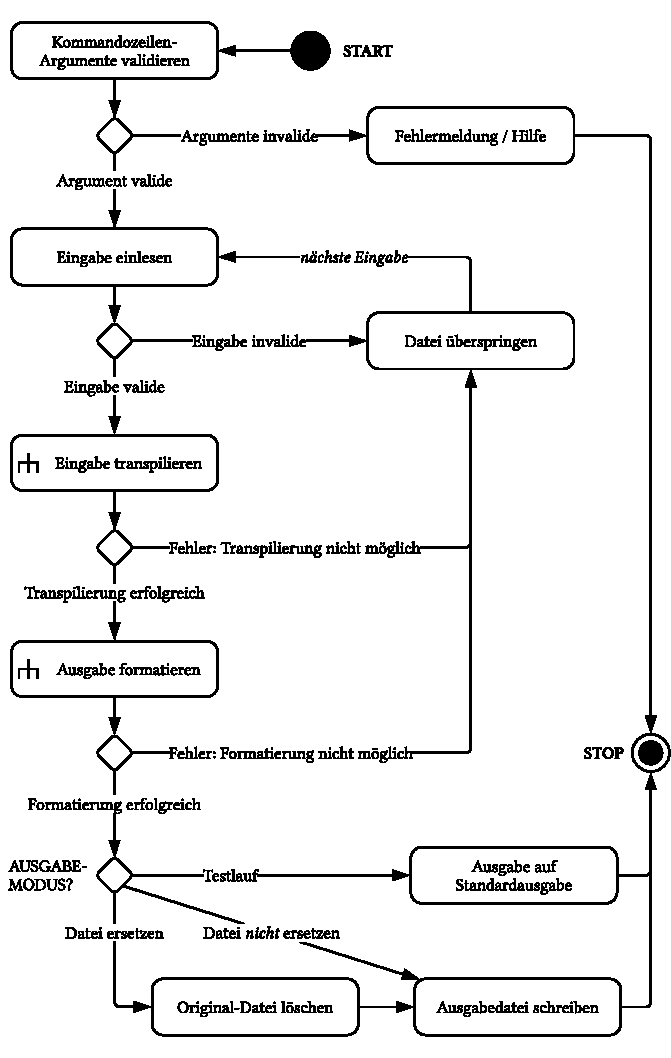
\includegraphics[width=0.85\textwidth]{src/4_Umsetzung/fig/activity-diagram-cli.pdf}
	\caption[Aktivitätsdiagramm des Kommandozeilenprogramms]{Aktivitätsdiagramm des Kommandozeilenprogramms. Vgl. eingebettete Diagramme~\ref{fig:activity-diagram-plugin} \enquote{Eingabe transpilieren} und~\ref{fig:activity-diagram-formatting} \enquote{Ausgabe formatieren}.}
	\label{fig:activity-diagram-cli}
\end{figure}

Abbildung~\ref{fig:activity-diagram-cli} auf Seite~\pageref{fig:activity-diagram-cli} zeigt das Aktivitätsdiagramm des Kommandozeilenprogramms. Als Erstes werden dessen Argumente eingelesen und validiert. Dabei wird überprüft, ob alle Eingabeverzeichnisse bzw. -dateien existieren und ob der Dateityp korrekt ist. Erlaubt sind lediglich JavaScript und JSX-Dateien. Sofern die Validierung fehlschlägt, wird die Anwendung mit einer Fehlermeldung beendet. Andernfalls wird daraufhin die Liste aller zu übersetzenden Flow-Dateien aufgebaut. Falls Verzeichnisse als Argument angegeben worden sind, so werden alle Dateien innerhalb dieser, die dem Wildcard-Muster für Eingabedateien entsprechen, zur Verarbeitungsliste hinzugefügt\footnote{vgl. Option \code{-{}-include-pattern}.}. Anschließend wird eine Schleife betreten, welche alle Elemente der Liste nach und nach verarbeitet. Da unsinnige Wildcard-Muster durch Benutzereingabe möglich sind, wird erneut überprüft, ob die aktuelle Eingabedatei valide ist. Sollte dies nicht der Fall sein, so wird diese übersprungen. Ansonsten wird der Quelltext der Datei durch den Parser von Babel eingelesen und so die Repräsentation des abstrakten Syntaxbaum des Programms erstellt. Daraufhin wird die Transpilierung durch das Babel-Plugin angestoßen. Auch hier kann es zu Laufzeitfehlern kommen, falls beispielsweise Syntaxfehler innerhalb des Eingabequelltexts vorliegen. In diesem Fall wird die aktuelle Datei ebenfalls übersprungen und eine Warnung ausgegeben.

Nachdem die Transpilierung abgeschlossen ist, wird der generierte TypeScript-Code unabhängig von Babel formatiert. Dabei wird eine selbst implementierte Funktion ausgeführt, die eine möglichst originalgetreuen Formatierung der Ausgabe umsetzt. Sollten unerwarteten Fehler auftreten wird auch hier die Datei gegebenenfalls übersprungen. Zuletzt kann der generierte TypeScript-Code ausgegeben werden. Dabei gibt es je nach Verwendung der Kommandozeilenoptionen drei Möglichkeiten: Sofern der Parameter \code{dry-run} gesetzt ist, wird das Resultat einfach auf die Standardausgabe geschrieben. Andernfalls werden neue TypeScript-Dateien im Verzeichnis der Eingabedateien erstellt. Falls die Option zum Ersetzen der Originaldateien angegeben wurde, so werden diese zuvor gelöscht.
Da die Verwendung von JSX-Syntax in TypeScript die Dateierweiterung \code{.tsx} vorschreibt~\autocite{TYPESCRIPT_HANDBOOK:JSX}, muss sicher gestellt werden, dass die Ausgabedateien die korrekte Endung erhalten. Analog müssen globale Typdeklarationen in Dateien mit der Erweiterung \code{.d.ts} geschrieben werden. Zur Bestimmung des korrekten Ausgabedateityps wird innerhalb des Babel-Plugins während der Transpilierung überprüft, ob JSX-Syntax in der Eingabedatei verwendet wird bzw. ob Typdeklarationen vorliegen. Hierfür werden Besucherfunktionen für diese speziellen AST-Knoten registriert, die eine Lookup-Tabelle aufbauen, welche die Abbildung der Originaldateien auf einen Ausgabetyp darstellt. Das Kommandozeilenprogramm kann diese Information anschließend beim Schreiben der Dateien abfragen und entsprechend reagieren.

\section{Formatierung des Ausgabequelltexts}
\label{sec:formatting}

Eine weitere Problematik, die sich während der Entwicklung des Transpilers gezeigt hat, ist die Formatierung des generierten Ausgabecodes. Weil Babel auf Grundlage eines \emph{abstrakten} Syntaxbaums arbeitet, liegt nach der Transformation des Programms keinerlei Information mehr über die ursprüngliche Formatierung des Codes vor. Im Gegensatz zu einem \emph{konkreten} Syntaxbaum, welcher der Ableitungsbaum einer formalen Grammatik ist~\autocite[45]{AHO:COMPILERS}, enthält der abstrakte Syntaxbaum lediglich \enquote{wesentliche Teile}~\autocite[21]{WALDMANN:PPS} davon. Infolgedessen geht die Einrückung und die Position der Leerzeichen und -zeilen in der TypeScript-Ausgabe verloren. Es hat sich weiterhin herausgestellt, dass auch die Position der Kommentare nach der Übersetzung nicht präzise beibehalten wird. Versuche mit der Option \enquote{\texttt{retainLines}}~\autocite{BABEL:GENERATOR} des Babel-Codegenerators, welche eine Beibehaltung der Zeilen in der Ausgabe bewirken soll, erzielten leider nicht das gewünschte Ergebnis. Auch nach Setzen dieser Eigenschaft unterscheidet sich das Format des generierten Quelltexts erheblich von der Eingabe. Da die möglichst originalgetreue Formatierung der Ausgabe eine der Anforderungen an den Transpiler ist\footnote{Vgl. Abschnitt~\ref{subsection:requirement:format}.}, wurde eine Formatierungsroutine implementiert, um diese Vorgabe unabhängig von Babel zu erfüllen. Diese wird nach der Transpilierung aller Eingabedateien durch das Kommandozeilenprogramm angestoßen (vgl. Abb.~\ref{fig:architecture-overview}) und im Folgenden erläutert. Um die Kommentare korrekt zu positionieren werden diese während der Transpilierung entfernt und nicht ausgegeben. Erst im Nachgang werden diese im Zuge der Formatierung in die Ausgabe eingefügt.

\begin{figure}[htb]
  \centering
  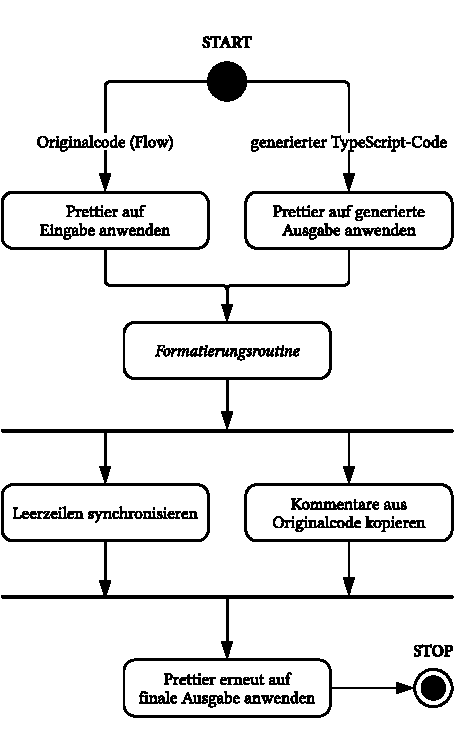
\includegraphics[width=0.55\textwidth]{src/4_Umsetzung/fig/activity-diagram-formatting.pdf}
	\caption[Aktivitätsdiagramm der Formatierung des Ausgabecodes]{Aktivitätsdiagramm der Formatierung des generierten Ausgabecodes.}
	\label{fig:activity-diagram-formatting}
\end{figure}

Der konzeptionellen Aufbau der Formatierungsfunktion wird in Abbildung~\ref{fig:activity-diagram-formatting} dargestellt. Deren Idee ist simpel: Nachdem sowohl die Ein- als auch die Ausgabe in einen vergleichbaren, konsistenten Zustand überführt worden sind, können Leerzeilen und Kommentare aus dem ursprünglichen Quelltext einfach übertragen werden. Konsistent bedeutet, dass sämtliche Ausdrücke und Anweisungen innerhalb beider Quelltexte die gleiche Zahl von Zeilen vereinnahmen, das heißt dass diese gleich umgebrochen werden. Diese Voraussetzung muss insbesondere auch für alle Flow-Konstrukte, nach deren Übersetzung nach TypeScript, gelten.
Grund für die Herstellung dieser Eigenschaft ist, dass das weitere Verfahren zeilenbasiert arbeitet, um die Originalformatierung in die Ausgabe zu übernehmen
Zur Herstellung eines solchen Ausgangszustand wird \textit{Prettier}~\autocite{SOFTWARE:PRETTIER} eingesetzt. Prettier ist ein Quelltext-Formatierer, der einen einheitlichen Programmierstil für Sprachen wie JavaScript, TypeScript, HTML und weitere ermöglicht.
Versuche haben gezeigt, dass die Ein- und Ausgabe bei Anwendung von Prettier aufgrund unterschiedlicher Syntax von Flow und TypeScript nicht in allen Situationen gleich umgebrochen wird. Deshalb wurde das Werkzeug geringfügig modifiziert, um eine größere Konsistenz der Ausgabe von Prettier zu erzielen\footnote{Siehe~\autocite{REFLOW_PRETTIER}.}.
Im ersten Schritt der Routine wird diese angepasste Version des Werkzeugs einerseits auf den Originalcode, andererseits auf den generierte TypeScript-Quelltext angewandt. Im Anschluss kann sukzessive über alle Zeilen der Eingabe iteriert werden, um in jedem Schleifendurchlauf zu prüfen, ob eine Leerzeile vorliegt. Gegebenenfalls wird diese an die entsprechende Position in der Ausgabe kopiert. Gleichzeitig werden Block- und Zeilenkommentare im ursprünglichen Flow-Programm gesucht und an die gleiche Stelle in den TypeScript-Code eingefügt. Auf diese Weise werden nach und nach alle Leerzeilen und Kommentare übertragen, sodass die originalgetreue Formatierung hergestellt wird. Zuletzt wird Prettier erneut auf die so entstandene Ausgabe angewandt, um verbleibende Probleme wie z.~B. doppelte Leerzeilen zu eliminieren.
